\documentclass[12 pt]{article}
\usepackage[utf8]{inputenc}
\usepackage{graphicx}
\PassOptionsToPackage{nottoc}{tocbibind}
\usepackage{tocbibind}
\usepackage[english]{babel}
\title{High Performance DSL's via OCaml}
\begin{document}
\begin{titlepage}
\begin{center}

% Upper part of the page. The '~' is needed because \\
% only works if a paragraph has started.
% 
\includegraphics[width=1\textwidth]{figures/nus_logo.jpg}\\[1cm]
\\[5cm]
\textsc{\Large B.Eng Dissertation}\\[0.3cm]
\textsc{\Large Project ID: H018570}\\[0.3cm]
\textsc{\Large 2014 - 2015}\\[0.3cm]

% Title
\HRule \\[0.4cm]
{ \huge \bfseries Embedded DSL for System Testing via Scala \\[0.4cm] }
\HRule \\[1.0cm]

% Author and supervisor
\noindent
\begin{minipage}{0.4\textwidth}
\begin{flushleft} \large
\emph{Submitted By:}\\
Rohit \textsc{Mukherjee}
A0091525H
\end{flushleft}
\end{minipage}%
\begin{minipage}{0.4\textwidth}
\begin{flushright} \large
\emph{Supervisor:} \\
Dr.~Chin Wei \textsc{Ngan}
\end{flushright}
\end{minipage}
\vfill

\vspace{8 mm}
In partial fulfilment of the requirements for the Degree of Bachelor of Engineering (Computer Engineering) National University of Singapore 
% Bottom of the page
\bigskip
% {\large \today}

\end{center}
\end{titlepage}
\maketitle

\vspace{-10 mm}
\tableofcontents

\newpage
\section{Abstract}
Domain-specific languages can provide a high-level user-oriented view for software development. Strongly-typed functional languages, like Scala, can provide a good platform for developing domain specific languages. DSLs contains the syntax and semantics that model concepts at the same level of abstraction that the problem domain offers. Over the semester, various techniques to develop high - performance DSLs have been explored using the Scala programming language. The domain chosen for developing the DSL is software system testing.
\bigskip

\noindent
There is a dearth of mature frameworks and tools available for system testing which can make the process painless and convenient. Throughout the course of this project, state of the art DSL design techniques coupled with powerful expressiveness and clean syntax of the Scala language are used to develop a DSL for system testing. This report takes a look at the key learnings, approaches taken, DSL developed so far and what it could be in the future.

\newpage
\section{Introduction}

\noindent
Domain specific languages provide a promising path to automatically compile code to parallel, heterogeneous and distributed hardware. However, in practice high performance DSLs still require considerable software expertise to develop and force users into tool-chains that complicate  prototyping and debugging \cite{delite}. The purpose of this project was to develop a DSL targeting a particular domain which was both performant, easy to use and easy to debug. The domain chosen for this project is that of software testing.

\subsection{Problem}
Testing is an integral part of software development. Unit Testing frameworks like JUnit, NUnit, TestNG and ScalaTest have been around for quite some time and allow software developers to conveniently and reliably test functionality in the form of Unit Tests. Proponents of "agile methodologies" highlight the importance of Test - Driven Development to ensure that the code base is well wrapped in tests and any sorts of regressions caused by code changes can be easily tracked and fixed \cite{tdd}. Test - Driven Development also prevents legacy code from being written, as comprehensive test suites are one of the best kinds of documentation code can come with.
\bigskip

\noindent
However, there is a scarcity of System Testing frameworks that allow developers to test the entire system with sample usage and match this behaviour against preset expectations. The availability of such a framework will allow developers to both ensure that their code has the correct functionality on a unit test level as well as a system level. In this project, a simple system testing DSL has been developed which allows quality analysts and system testers to write test cases in a declarative, natural language like syntax and gather test statistics on what tests failed. This allows a higher level of abstraction when it comes to testing and allows them to write exhaustive test cases without concerning themselves much with code.

\subsection{Solution}
In this project, some of the different ways scalable, high - performance DSLs could be written were examined and evaluated. Over the course of this project, a domain specific language for system testing was developed. The language allows users to create test suites and cases in a declarative manner and also declare custom output matchers. The system currently deals with testing systems as a whole but may be extended in the future to have greater granularity.

\subsection{Project Objectives/Goals}
The DSL developed during the course of this project had the primary objective of software system testing. System testing of software is testing conducted on a complete, integrated system to evaluate the system's compliance with its specified requirements. The requirements for the DSL were:
\begin{itemize}
\item Testing systems with inputs and matching against specified outputs
\item Testing whether the system is functional as a whole and generates output
\item Intuitive, declarative syntax for testers
\item Ease of debugging and use
\item Extensibility of the DSL
\item Ease of integration with application code
\end{itemize}

\newpage
\section{Literature Review}
There are several ways of designing and implementing Domain Specific Languages, each way having several merits and demerits. One of the most fundamental ways of classifying DSLs are Internal and External. \textbf{Internal DSLs} use the infrastructure of existing programming languages and build domain - specific constructs on top it. \textbf{External DSLs} are developed ground up and has separate infrastructure for lexical analysis, parsing, interpretation and compilation. In this project, we are restricting ourselves to internal or embedded DSLs on the host language of Scala.
\bigskip

\subsection{Domain Specific Language Design}
Ghosh discusses two approaches to constructing internal DSLs - \textbf{Embedded} and \textbf{Generative} \cite{dslsInAction}. Statically typed languages offer types as one of the means to abstract domain semantics and make the surface syntax of the DSL concise. Typed models come with a
guarantee of some level of implicit consistency in the programming model. The biggest advantage of this technique is that because the DSL’s type system is embedded in the type system of the host language, the type system is automatically type-checked by the language compiler. This approach means that DSL users are able to use the IDE for debugging and tooling. In our System Testing DSL, this embedded DSL approach has been explored.
\bigskip

\begin{figure}[h!]
  \centering
    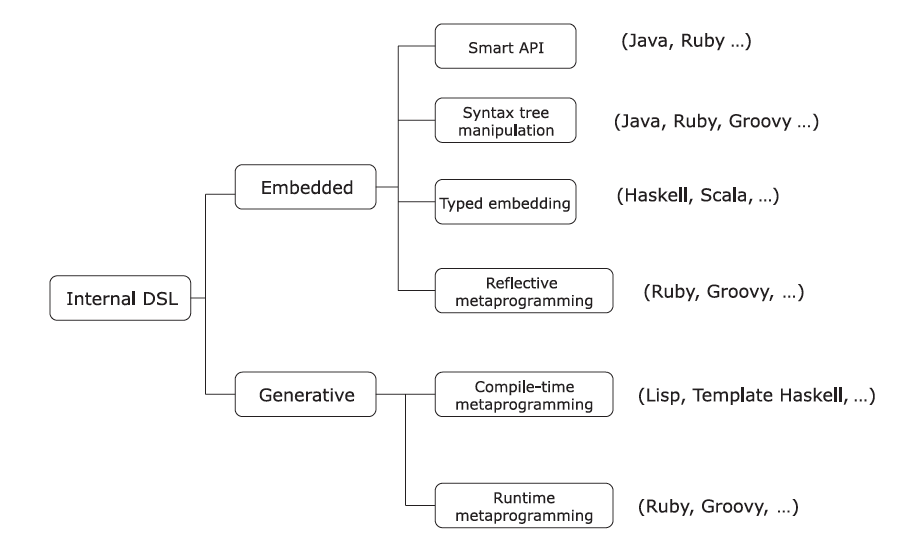
\includegraphics[height=200px]{figures/classification.png}
  \caption{Micro - classification of DSLs}
\end{figure}

\noindent
Languages like Haskell and Scala offer advanced static typing with type inference allowing DSL developers to write embedded DSLs without having to resort to code generation techniques, pre - processors or macros. As a DSL user, type abstractions can be composed directly. This is the approach that has been taking while writing the System Testing DSL. Ghosh talks about using method chaining and fluent interfaces in DSL development as this gives a finished, declarative, natural language like feel \cite{fluentInterface}. The builder pattern is one more way in which DSL's can be made more expressive to the domain user. The builder pattern along with method chaining have been incorporated into the System Testing DSL to provide ease of use and expressiveness.

\subsection{Lightweight Modular Staging: A run - time code generation approach}
Rompf and Odersky (2010) talk about an alternative approach to writing DSLs in Scala using a run - time code generation approach called lightweight modular staging \cite{lms}. This approach involves both a generative and an embedded approach. The DSL is provided as a library and involves run - time code generation in different stages. The approach is called \textbf{Light - Weight Modular Staging (LMS)}. The approach is lightweight because the whole framework is implemented as a library and the staged code is very shallowly embedded into the program generator. Some of the features of lightweight modular staging are described below:
\begin{itemize}
\item Immediate/deferred compilation of certain objects are distinguished by type
\item The Scala language is expressive enough to allow the framework to be implemented as a library
\item staged code is “very shallowly” embedded into the program generator
\end{itemize}
\bigskip

\noindent
Lightweight modular staging provides many of the benefits of using a dedicated multi-stage programming language such as MetaOCaml, in particular concerning well-formedness and type safety, but goes beyond that in systematically preventing code duplication and providing a clean interface for incorporating generic and customized optimizations.

\subsection{Delite: A framework for high - performance DSL's}
A third approach to writing embedded, high - performance DSLs conducted by Odersky built upon the concept of using lightweight modular staging. The research resulted in a framework called Delite \cite{delite}. Delite's compilation pipeline takes care of optimizing for target hardware such as multi - core processors, GPUs and computing clusters.

\begin{figure}[h!]
  \centering
    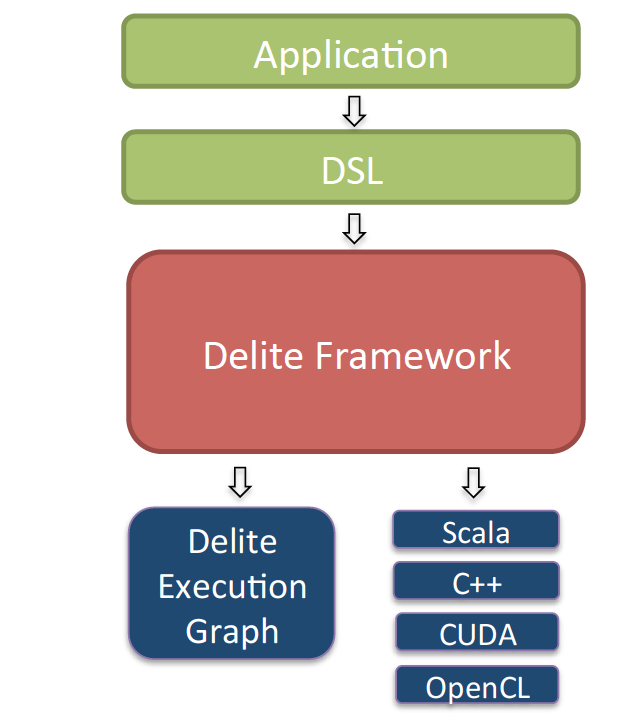
\includegraphics[width=170px]{figures/delite.png}
  \caption{Delite Framework Overview}
\end{figure}

\noindent
In the early stages of this project, the Delite framework was experimented with to gauge the suitability of the framework in everyday DSL development. However, due to the lack of sufficient tooling and documentation - the plans of using Delite were set aside till the next semester of research so that better support and documentation is available.
\bigskip

\subsection{Approach Chosen}
Out of the three approaches explored - \textbf{DSL development using embedded types}, \textbf{Lightweight Modular Staging} and \textbf{The Delite Framework}, the first one was chosen for developing the System Testing DSL this semester. The choice was made so that we could gain an understanding of the types and usage required in the DSL and then look into lower level code optimizations in the following semester.
\newpage

\section{Progress Report}

\subsection{Repository}
The code for this project and related documentation can be found in the repository below on the master branch.\newline
\textbf{Link:} https://github.com/rohitmukherjee/High-Performance-DSLs

\subsection{Overview of Progress}
Over the course of this semester, a DSL for system testing was developed using Scala as the host language. It can be used for testing any set of executables/applications and match their generated console output against specified values. The language can also be used to check whether the system is operational or not.
\bigskip

\noindent
The DSL has a declarative, natural language like syntax. A snippet below shows how to run Sleek Tests and match against expected output.

\begin{figure}[h!]
  \centering
    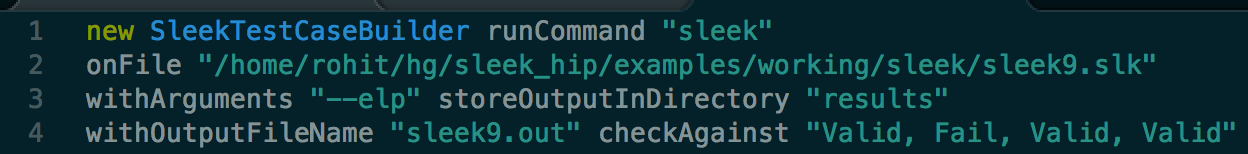
\includegraphics[height=50px]{figures/code_snippet_1.png}
  \caption{An example of the DSL syntax}
\end{figure}

\subsection{Design Choices}

Some of the primary design choices in the project are summarized below:

\begin{itemize}
\item \textbf{Choice of Approach 1(Internal, Embedded DSL with no staging)}: Instead of starting off development using the Delite Framework or the Lightweight Modular Staging Library, I decided to write a DSL with an embedded type system and no run - time code generation or optimizations. This allowed me to understand the important types and constructs required in the domain and develop a clean syntax. It also allowed me to model the domain without concerning myself with lower level optimizations prematurely.

\item \textbf{Choice of Scala as host language}: The adoption of Scala has grown tremendously over the last 5 years in the industry with large organizations such as Twitter, Bank of America Merrill Lynch and Groupon using it for DSL design \cite{scala}. The expressive syntax and intelligent type inference allows a clean domain syntax and type system to be developed. Portability of code because of the JVM platform is another factor promoting Scala's adoption \cite{scala}. The reasons for using Scala are summarized below:

\begin{figure}[h!]
  \centering
    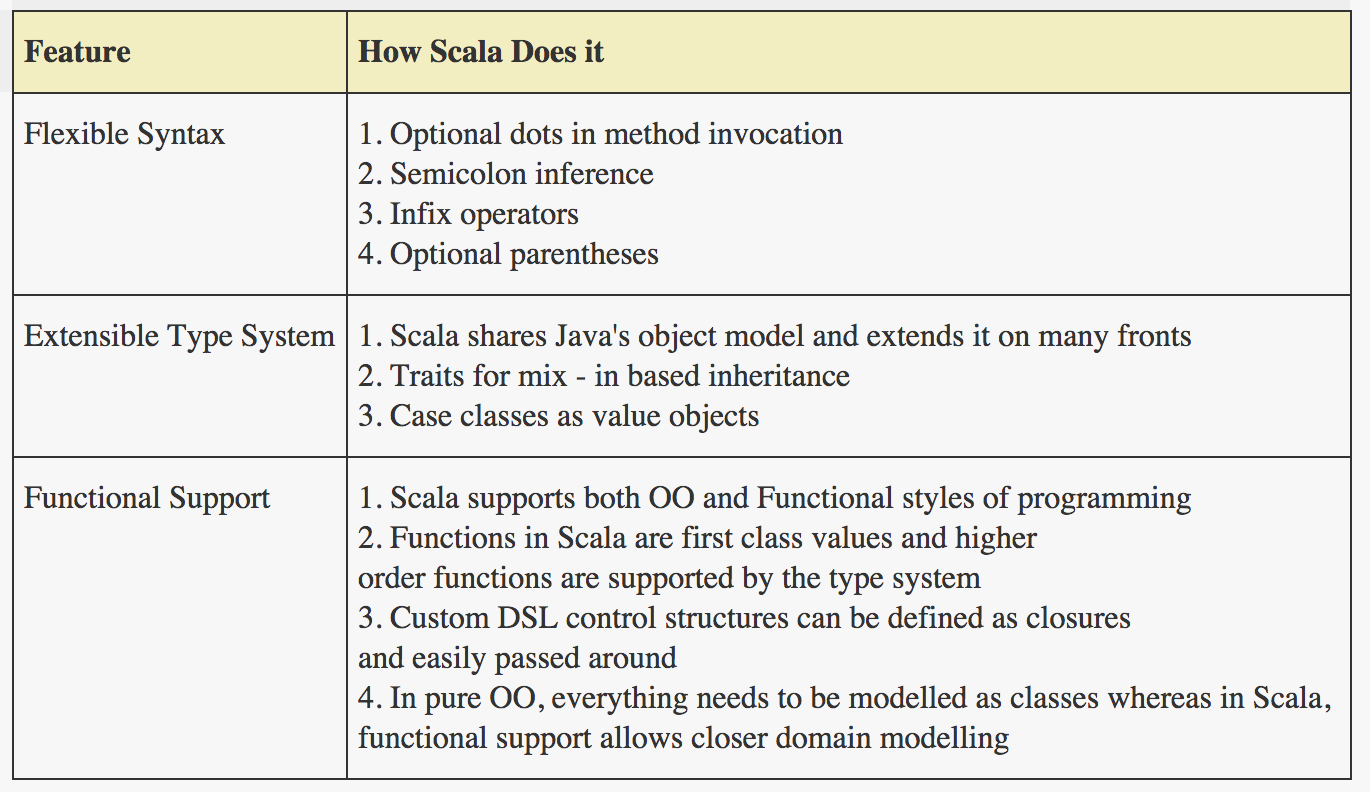
\includegraphics[width=400px]{figures/scala_motivation.png}
  \caption{Motivation for using Scala}
\end{figure}

\end{itemize}
\subsection{Design Pattern Choices}

Ghosh \cite{dslsInAction} talks about certain design patterns being industry "best - practices" for DSL development. Over the course of this project, these patterns have been used extensively:
\begin{itemize}
\item \textbf{Singleton Pattern} - For re - usable components like regex/file sytem utilities
\item \textbf{Builder Pattern} - For creating a declarative, natural language like syntax
\item \textbf{Factory Pattern} - For context - aware choice of which kind of class to instantiate
\end{itemize}

\noindent
Fowler's concept of the "Fluent Interface" can be extended to Scala which models behaviour using traits rather than interfaces \cite{scala}. This in conjunction with the builder pattern lead to a declarative syntax. One of the uses of the builder is shown below.

\begin{figure}[h!]
  \centering
    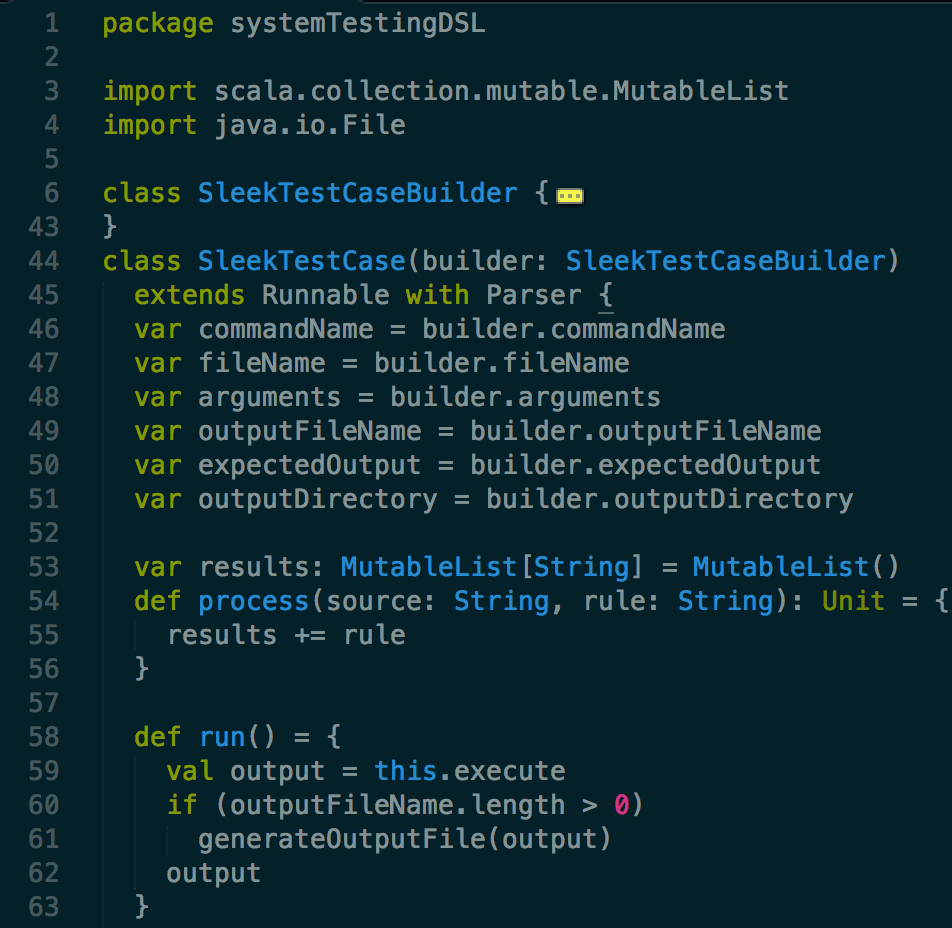
\includegraphics[width=300px]{figures/builder_pattern.png}
  \caption{An example of builder pattern usage}
\end{figure}

\subsection{Overview of Code}
\begin{itemize}
\item package systemTestingDSL
    \begin{itemize}
        \item \textbf{Trait Runnable} - Models behaviour of any executable/command that can be run
        \item \textbf{Case Class General Runnable} - Models implementation of any executable/command 
        \item \textbf{Trait Parser} - Mix - In containing methods for matching and parsing test output
        \item \textbf{Case Class SleekTestCase} - Test Case especially for Sleek verification
        \item \textbf{Case Class TestCase} - Any Test Case
        \item \textbf{Case Class GenericTestSuite} - Automated testing of files of a certain type found          using regex matching
        \item \textbf{Object Usage} - Demonstrates usages of DSL developed
    \end{itemize}
\item package systemTestingDSL.fileSystemUtilities
    \begin{itemize}
        \item Singleton object performing file matching/reading/writing and output generation
    \end{itemize}
\item package systemTestingDSL.matchers
    \begin{itemize}
    \item \textbf{Trait Matcher} - Models behaviour for any generic matcher
    \item \textbf{DiffMatcher} - Matches two files based on their diff
    \end{itemize}
\end{itemize}

\subsection{Functionality Completed}
Currently the DSL has the following features:
\begin{itemize}
\item Construct test cases for individual systems against expected output
\item Run tests for all test files in a directory against previously generated output
\item Custom matchers based on regex and diff
\item Declarative syntax
\end{itemize}
\subsection{Thoughts on preliminary investigation}
The following conclusions were drawn from the initial investigation:
\begin{itemize}
\item Scala provides a friendly ecosystem to write DSLs in many ways (as discussed)
\item System Testing is a domain that could use greater automation and tooling and the objective of our DSL is make it easier to test systems
\item A substantial amount of research is being conducted in making the Scala compilation pipeline more DSL friendly and in abstracting away target hardware specific optimization
\item Application of appropriate design patterns and good syntactical rules help construct DSLs with a clean, easy to use API
\end{itemize}


\subsection{Usage}
The project is built using the Simple Build Tool (sbt) and can be set up by executing the \textit{run} target \cite{sbt}. SBT was used because it is commonly used in industry to build and manage dependencies in Scala projects. It exports the compiled sources in .jar format allowing easy use in the form of a library.

\newpage
\section{Research Plan}
The goal for this semester was to read and apply the methods mentioned in literature and build a DSL that can be used for system testing. This process helped understand some of the patterns that can be applied in internal DSLs, requirements and specifications of the DSL itself and usage scenarios.
\bigskip

\noindent
The broad goals for next semester will be to apply some optimization techniques to improve performance of the DSL and also extract it to a more general purpose of testing. The research goals for the next semester are as follows:
\begin{itemize}
\item Improve performance through usage of Delite pipeline or other run - time code optimization techniques
\item Extend suite of functionality to include more kinds of tests such as
    \begin{itemize}
    \item Performance Tests
    \item Unit Tests
    \item Integration Tests
    \end{itemize}
\item Greater automation and flexibility as far as test execution is concerned
\item Cleaner syntax and idioms
\item Ease of integration with existing software projects for testing purposes
\end{itemize}
\bigskip

\noindent
A tentative time - line for the aforementioned research plan is shown below:
\bigskip
\centerline{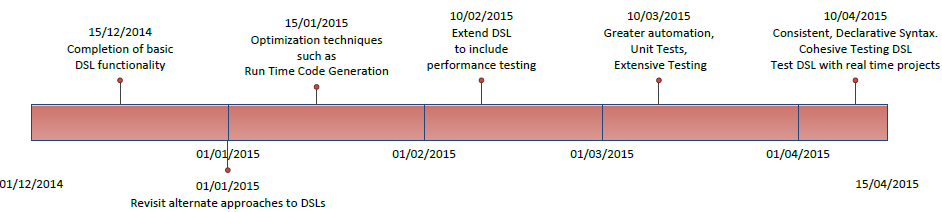
\includegraphics[width=600px]{figures/timeline.png}}

\newpage
\begin{thebibliography}{9}

\bibitem{fluentInterface} Fowler, M. (2005, 12 20). Fluent interface. 
Retrieved from http://martinfowler.com/bliki/FluentInterface.html

\bibitem{dslsInAction}Ghosh, D. (2011). DSLs in Action (1st ed., pp. 20 - 87). Connecticut: Manning.

\bibitem{tdd} Introduction to Test Driven Development (TDD). (n.d.). Retrieved November 4, 2014.

\bibitem{lms} Odersky, M., \& Rompf, T. (n.d.). Lightweight Modular Staging: 
A Pragmatic Approach to Runtime ode Generation and Compiled DSLs. \textit{GPCE 2010, October 10–13, 2010}. Retrieved from http://infoscience.epfl.ch/record/150347/files/gpce63-rompf.pdf

\bibitem{delite} Odersky, M., \& Sujeeth, A. (2013). Forge: Generating a 
High Performance DSL Implementation from a Declarative Specification. \textit{GPCE 2013: 12th International Conference on Generative Programming: Concepts \& Experiences}. 
Retrieved November 4, 2014, from http://ppl.stanford.edu/papers/gpce13-sujeeth.pdf

\bibitem{sbt} The interactive build tool (sbt) http://www.scala-sbt.org/
\bibitem{scala} The Scala Programming Language (The Scala Programming Language)
http://www.scala-lang.org/
\end{thebibliography}
\end{document}